\begin{figure}[htbp]
\centering
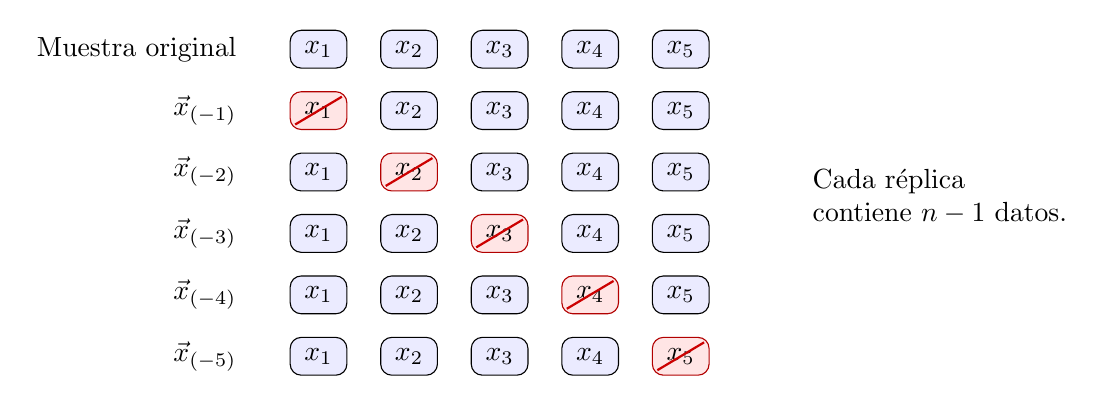
\begin{tikzpicture}[x=1.15cm,y=0.78cm,
  dato/.style={draw,rounded corners,minimum width=0.72cm,minimum height=0.48cm},
  omitido/.style={dato,fill=red!10,draw=red!70!black}]
  \node[anchor=east] at (-0.8,0) {Muestra original};
  \foreach \i in {1,...,5} {
    \pgfmathtruncatemacro{\pos}{\i-1}
    \node[dato,fill=blue!8] at (\pos,0) {$x_{\i}$};
  }
  \foreach \r in {1,...,5} {
    \pgfmathtruncatemacro{\y}{-\r}
    \node[anchor=east] at (-0.8,\y) {$\vec{x}_{(-\r)}$};
    \foreach \i in {1,...,5} {
      \pgfmathtruncatemacro{\pos}{\i-1}
      \ifnum\i=\r
        \node[omitido] (omit-\r) at (\pos,\y) {$x_{\i}$};
        \draw[red!80!black,thick] ([xshift=2pt,yshift=2pt]omit-\r.south west) -- ([xshift=-2pt,yshift=-2pt]omit-\r.north east);
      \else
        \node[dato,fill=blue!8] at (\pos,\y) {$x_{\i}$};
      \fi
    }
  }
  \node[anchor=west,align=left] at (5.35,-2.4)
    {Cada réplica\\ contiene $n-1$ datos.};
\end{tikzpicture}
\caption{Jackknife de eliminación individual para una muestra de tamaño cinco. En cada fila se excluye, por turno, una observación distinta.}
\label{fig:jackknife-muestras}
\end{figure}